\chapter{Methodology}

\section{Aims and Objectives}

The key objectives of this project are:

\begin{enumerate}
    \item To develop the necessary tools to process the raw recorded data and extract the demodulated baseband.
    \item Develop a software tool to generate an MSK waveform to allow for in depth investigation
    \item Using information extracted from the real recorded data develop a tool to simulate the atmospheric noise that appears in the real world signals.
    \item Develop an algorithm that can extract the symbols from a demodulated MSK signal and improve the BER using non-data related methods.
\end{enumerate}

The key aims are:

\begin{enumerate}
    \item Investigate the signal properties from VLF transmitters around the globe listed in \ref{tab:vlftransmitters}. 
    \item Compare these properties to the simulated signals generated.
    \item Investigate how different types of noise can affect the BER associated with a particular transmission.
    \item Suggest how this BER may be improved and the impact of atmospheric noise mitigated
\end{enumerate}
\section{Introduction to Methodology}
The investigation in order to achieve the aims of this project will contain two principle components. 
\begin{enumerate}
    \item \textbf{Simulation}
    
    The purpose of this is to develop simulation tools that allow for the generation of MSK signals in a controlled environment, in order to best replicate signals in the real world where there is a known bit structure and noise content. In this instance the particular importance of them is that the original bit sequence is a known quantity compared to the data recordings where the bit sequence can only be estimated. 
    
    \item \textbf{Analysis}
    
    This relates to the study and investigation of the signal characteristics. This analysis will be applied to both the real data and the simulation data. This will allow for objective performance metrics to be developed in order to assess the performance of algorithm.
\end{enumerate}


\section{Stage 1: Development of Understanding} 
The importance of developing a good simulation tool is essential in order to assess the performance of the final algorithm. There are unknowns regarding the real data, which limits the ability to accurately and reliably compare results. Therefore, to be able to create like for like simulations with known quantities is essential.
\\\\
The first stage involves an investigation into the real recording already present. In order to develop an understanding of the real data to help validate the later stages. Particular techniques used include the the use of the Fast Fourier Transform which is the computationally efficient implementation of the Fourier Transform.
\\\\
This stage involved the basic steps of signal receptions, and developing these software tools for use later on:

\begin{enumerate}


    \item \textbf{Filter} 
    
    The use of a rectangular filter in the frequency domain is the choice for this operation as it offers zero phase shift. Potential downsides are high frequency 'flutters' present at the temporal extremes of the data however this negates the requirement for a detailed investigation into the phase response of various filters. On the assumption that this rectangular filter can be considered an ideal bandpass filter.

    \item \textbf{Downconvert}

            Downconversion is the process of removing the carrier frequency. This is generally achieved as illustrated by Figure \ref{fig:downconversion} and described mathematically by Equation \ref{eq: downconversion}. In the frequency domain this produces a spike at 0 and $2f_c$.
            \begin{equation}
                d(t) = s(t) e^{2 \pi f_c t j}
                \label{eq: downconversion}
            \end{equation}

    \item\textbf{ Low Pass Filter} 

            Another box car filter to extract the baseband signal from the complex multiplication. This is necessary to remove the peak at $2f_c$, that results from the multiplication with the complex sinusoid.

    \item \textbf{Decimate}

            At this stage it is also possible to decimate, which is in effect downsampling the signal. The advantage of this is that it can reduce the amount of data required for a signal. However a result of downsampling is that part of the process is removing information from the signal. For the purpose of this exercise downsampling is avoided unless absolutely necessary.

    \item \textbf{Demodulate}

            It is important to remember that the carrier is phase modulated, therefore
            we are interested in extracting the phase of the baseband signal. This is achieved through differential demodulation, (\cite{DSP101}) If we call baseband b(t), demodulation is shown by Equations \ref{eq:instphase}a,b and c.
            \begin{subequations}
                \begin{equation}
                    \angle b(t) = arctan\left(\frac{Im[b(t)]}{Re[b(t)]}\right) = \phi
                    \label{eq:atanPh}
                \end{equation}
                \begin{multicols}{2}
                
                \begin{equation}
                    \phi = \omega t = 2\pi f
                    \label{eq:omega}
                \end{equation}
                \begin{equation}
                    \frac{d}{dt}\phi = \omega
                    \label{eq:instfeq}
                \end{equation}
                \end{multicols}
                \label{eq:instphase}
            \end{subequations}
            It is important to note that the instantaneous phase will be in the range of $pi \rightarrow -pi$, therefore it is necessary to unwrap the phase before differentiating it. This is the process of changing point where there is a jump greater than $\pi$ to the $2\pi 's $ complement. This prevents the large jumps from dominating the differential.
        
        \end{enumerate}


\begin{figure}[h!]
    \centering
    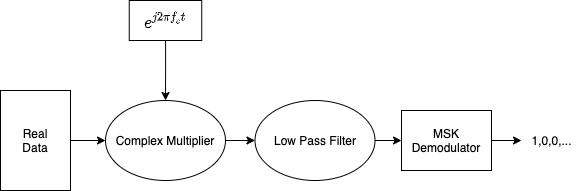
\includegraphics[width = \textwidth]{figs/method/downconversion.png}
    \caption{Passband to Baseband Conversion}
    \label{fig:downconversion}
\end{figure}

The real data used consists of two seconds of data recorded using a sampling frequency of 1\si{\mega\hertz}. This stage of the exercise is to establish which of many VLF transmitters around the world are present in the recording (\cite{wikipediaVLF}). The transmitters that are expected to be received are shown by Table \ref{tab:vlftransmitters}.

\begin{table}[h!]
\centering
\begin{tabular}{l|l|c}
\textbf{Callsign} & \textbf{Location}    & \textbf{Centre Frequency $f_c$ [kHz]} \\
\hline 
GQD               & Anthorn, UK          & 19.6                            \\
ICV             & Tavolara, Italy & 20.27 \\
HWU               & Saint-Assise, France & 20.9                            \\
GZQ               & Skelton, UK          & 22.1                            \\
DHO38             & Rhauderfehn, Germany & 23.4                            \\
NAA               & Cutler, Maine USA    & 24.0                             
\end{tabular}
\caption{Table of active VLF transmitters}
\label{tab:vlftransmitters}
\end{table}

This stage of the process is important to understand the nature of the real signals. The aim was to develop a full understanding of the signals that we are aiming to simulate and ultimately the real signals that the aim is to recover completely. Regarding the simulation the output of this step is to create metrics which can be used to help design, validate and improve simulation tools.

An additional dataset is also available for comparison that was recorded at a time when there was little to no lightning. This was again recorded at a rural location to minimise the presence of Gaussian noise.

\section{Stage 2: Software Design}
In order to simulate this particular problem it has been broken into 2 separate stages.
\subsection{Carrier Generation}
The MSK carrier signal is described by Equation \ref{eq:mskcarrier}. The message is split into even and odd information ie. even and odd bits, encoded as 1 or -1 corresponding to 1 or 0. These become the In Phase and Quadrature components respectively. Each bit pulses for $2T_b$ which is equivalent with the even bits pulsing on -T, T, 3T etc and the odd bits pulsing on 0, 2T, 4T etc. These odd and even signals then have to be encoded into $a_I$ and $a_Q$ these are the modulating pulse. Both I and Q can be considered sine waves as I simply leads Q by $\frac{\pi}{2}$. The important thing to note is that the phase doesn't change every symbol, but only when there is a sign change of the symbol.
These can then be used to pulse-shape, the sideband frequencies. The expected instantaneous frequency can be easily inferred from the bandwidth. Because $T_b = \frac{1}{BW}$ the frequency of the I and Q pulses is $f_{pulse} = \frac{1}{2BW}$ hence $f_{dev} = \pm\frac{f{pulse}}{2}=\pm\frac{BW}{4}$. Combining all these elements together allows for the definition of a frequency modulated carrier $s(t)$ defined by Equation \ref{eq:mskcarrier}.


\begin{equation}
s(t) = \underbrace{a_I cos\left(\frac{\pi t}{2T_b}\right)}_{\text{I Component Cosine Pulse}}\underbrace{cos(2\pi f_ct)}_{\text{Cosine Carrier}} + \underbrace{a_Qsin\left(\frac{\pi t}{2T_b}\right)}_{\text{Q Component Sine Pulse}}\underbrace{sin(2\pi f_ct)}_{\text{Sine Carrier}}
\label{eq:mskcarrier}
\end{equation}

\subsection{Noise}
\subsubsection{Impact of Noise}
As previously mentioned the recorded signal can be considered as being composed of three components. The received signal is the sum of all these signal components and they can all be considered as complex sinusoids. As background Gaussian noise is fairly easy to predict it is being ignored for the purposes of this investigation. This leaves the two components left as the transmitter and the impulsive lightning noise. 
\\\\
Each of the two components is complex and can be represented generally by Equations \ref{eq:complexEqs}. This is a phase modulation method, the extraction process for this has been defined by Equation \ref{eq:atanPh}. This considers the extracted baseband as a single signal, whereas in reality it has multiple components. The addition process in complex numbers can result in a phase change, especially if the two values are in different quadrants of the complex plane. Equation \ref{eq:sumSig} shows the phase calculation of the constituent components, if the magnitude of the lightning is much greater than that of the transmitter this could have a large affect on the apparent phase angle of the signal. 

\begin{subequations}
\begin{equation}
    y(t) = Ae^{j2\pi f t}
    \label{eq:complexsine}
\end{equation}
\begin{equation}
    y(t) = A(cos(2\pi ft) + jsin(2\pi ft))
    \label{eq:complexsine2}
\end{equation}
\label{eq:complexEqs}
\end{subequations}

\begin{subequations}
\begin{equation}
    b(t) = r(t) + n(t)
\end{equation}
\begin{equation}
    \angle b(t) = \arctan\left(\frac{Im[r(t)]+Im[n(t)]}{Re[r(t)]+Re[n(t)]}\right)
    \label{eq:sumSig}
\end{equation}
\end{subequations}
\subsubsection{Noise Generation}
Following on from the generation of a suitable carrier signal it needs to be corrupted with noise of similar characteristics. As stated by \cite{Chrissan2000} this can be modelled using a statistical model. However, as for this investigation there is data available containing an unusual amount of lightning activity this can be used to create Amplitude Probability Distribution, using the absolute amplitude of the complex trace. The complex amplitude for a signal s(t) is calculated using Equation \ref{eq:complexAmp}.

\begin{equation}
    A = \sqrt{Re[s(t)]^2 + Im[s(t)]^2}
    \label{eq:complexAmp}
\end{equation}

A discrete PDF can be developed by creating a histogram from this data using numpy's histogram method. This method uses the maximum of the Sturges or the Friedman-Diaconis method in order to determine bin number and width\footnote{\hyperlink{https://numpy.org/doc/sTable/reference/generated/numpy.histogram.html}{https://numpy.org/doc/stable/reference/generated/numpy.histogram.html}}.
This histogram corresponds to the APD for the signal. Normalising the histogram to a unit interval allows the creating of a cumulative distribution function(CDF). Once a CDF has been created, by generating a random probability an absolute amplitude value can be extracted from the CDF.


\section{Stage 3: Algorithm Development}
Following on from the successful development of a simulation tool the next stage is the development of an algorithm. The purpose of this is to ultimately extract the symbols from the real signal, which is developed and tested using the simulated waveforms.
\\
The principle of the algorithm is based on several known conditions. The process of downconversion makes the carrier frequency of the signal zero leaving only the modulating waveform. The range of the instantaneous frequency for this waveform can be used to determine the bandwidth of the signal and in turn the time per symbol $T_b$, from this the approximate number of symbols can be estimated. A symbol change ie 1 to -1 or vice versa will be observed by the signal crossing the zero axis. Using the time difference in between zero crossing the number of symbols in that interval can be determined. 

\section{Stage 4: Testing and Evaluation}
The final stage of the investigation is to combine the developed tools in order to investigate the performance of the developed algorithm. The aims of this is to assess the breakdown point of the algorithm by simulating different scenarios with different types of noise. Using each of these scenarios the breakdown points can be analysed alongside the signal characteristics in order to develop a strategy to mitigate against bit loss.
\subsection{Investigations}\label{sec:investigations}
Several investigations need to be carried out in order to assess the limitations of symbol recovery. The main judge of this is the BER as previously mentioned is the number of incorrectly estimated symbols per transmission. This is shown by Equation \ref{eq:ber}. This is a simple exercise when using simulated signals as the initial message and received message are known so it is a simple comparison exercise. However for the real data the extracted bits are known and the expected total number of bits can be calculated, the original transmitted however is not known. An estimate of the BER can be calculated by looking at the net displacement of the phase, because for a 1 the phase has a positive gradient and for a 0 the phase has a negative gradient. If the final displacement is positive then there are more 1's, if the final displacement is negative then there are more 0's in the message. Finally if it is zero then there are equal 1's and 0's. The difference in number of each symbol can be calculated using Equation \ref{eq:delSym}. Then using Equations \ref{eq:Nbits}, \ref{eq:N1s} and \ref{eq:N0s}, the quantities of each symbol can be estimated. Then the No. of incorrect bits present can be determined by using either Equation \ref{eq:errbit1} or \ref{eq:errbit0}. This method is purely developed to provide an estimate of BER within the real signal. The big assumption that it makes is that the final recording made is at a point in the time series where there is no noise and therefore the phase at the point represents the phase displacement of the transmitter phasor. A further assumption is that after a lightning event the signal returns to that of the transmitter. This metric is very much an estimate as two errors on opposite symbols cancel each other out. This limitation is the driving reason why this metric is a useful reference but it is not robust enough to quantify the performance of any bit recovery algorithm. 

\begin{multicols}{2}
\begin{equation}
    \text{BER} = \frac{\text{Incorrect No. Bits}}{\text{Total No. Bits}}
    \label{eq:ber}
\end{equation}
\begin{subequations}
\begin{equation}
    N_{\text{bits}} = \frac{T_{\text{total}}}{T_{\text{b}}}
    \label{eq:Nbits}
\end{equation}
\begin{equation}
    \Delta_{\text{sym}} = \frac{\frac{\phi_{\text{final}}}{2\pi}}{\frac{BW}{4}T_b} = \frac{2}{\pi}\phi_{\text{final}}
    \label{eq:delSym}
\end{equation}
\begin{equation}
    N_{\text{1's}} = \frac{N_{\text{bits}} + \Delta_{\text{sym}}}{2}
    \label{eq:N1s}
\end{equation}
\begin{equation}
    N_{\text{0's}} = \frac{N_{\text{bits}} - \Delta_{\text{sym}}}{2}
    \label{eq:N0s}
\end{equation}
\begin{equation}
    \text{Incorrect Bits} = \text{N}_{\text{1's-Estimated}} - \text{N}_{\text{1's-Extracted}}
    \label{eq:errbit1}
\end{equation}
\begin{equation}
    \text{Incorrect Bits} = \text{N}_{\text{0's-Estimated}} - \text{N}_{\text{0's-Extracted}}
    \label{eq:errbit0}
\end{equation}
\label{eq:berEst}
\end{subequations}
\end{multicols}
To assess the absolute performance of the symbol recovery algorithm including it's limitations, noise level needs to be quantified. This is done using the signal to noise ratio, defined by Equation \ref{eq:snr}, where P represents power. When assessing frequency modulation methods energy density per bit per power spectral density can be used. This is defined by Equation \ref{eq:ebN01}, where $f_b$ is the bitrate.
\begin{multicols}{2}
\begin{subequations}
\begin{equation}
    \text{SNR} = 10log_{10}\left(\frac{P_{\text{transmitter}}}{P_{\text{noise}}}\right)
    \label{eq:snr}
\end{equation}
\begin{equation}
    P_{\text{signal}} = \frac{\sum_{t=0}^{N} s(t)^2}{T_{signal}}
    \label{eq:psignal}
\end{equation}
\begin{equation}
    P_{\text{transmitter}} = P_{\text{signal}} - P_{\text{noise}}
\end{equation}
\end{subequations}

\begin{equation}
        \frac{E_b}{N_0} =  \frac{P_{\text{transmitter}}}{P_{\text{noise}}} \frac{BW}{f_b}
        \label{eq:ebN01}
\end{equation}
\end{multicols}
The simulated signal noise power is easy to calculate by subtracting the power of the carrier away from the power of the noise corrupted signal. However in order to estimate the SNR of the real recorded data it is necessary to make an estimate of the noise. In statistical terms the noise can be considered as the outliers of the data. Outliers can be defined as all points that lie outside of the range of the data. Equations \ref{eq:Q1} and \ref{eq:q3} are used to calculate the \nth{25} and \nth{75} percentile of the data. The interquartile range (IQR) is the difference between the two values, shown by Equation \ref{eq:iqr}, this is a widely used method to assess the spread of data that is not normally distributed. It is clearly established in the literature that signals within this band are not. Working on the assumption that the amplitude of the transmitter should represent a grouping, it can be deduced that any amplitude values outside this grouping can be considered noise. This grouping is defined as all the values that sit in between an upper and lower limit. The range limits are then determined by Equations \ref{eq:upplim} and \ref{eq:lowlim}. Any data that lies outside these points is then considered noise. This statistical analysis is applied to the absolute amplitude of the complex sinusoid received.

\begin{multicols}{2}

\begin{subequations}
    \begin{equation}
        y(t) = |s(t)|
    \end{equation}
    \begin{equation}
        \text{Q1} = \text{median}\left(y_{0},y_{1},\dots,y_{\frac{N}{2}}\right)
        \label{eq:Q1}
    \end{equation}
    \begin{equation}
        \text{Q3} = \text{median}\left(y_{\frac{N}{2}},y_{\frac{N}{2}+1},\dots,y_{N}\right)
        \label{eq:q3}
    \end{equation}
    \begin{equation}
        IQR = Q3 - Q1
        \label{eq:iqr}
    \end{equation}
    \begin{equation}
        \text{Lim}_{\text{upper}} = Q3 + k IQR
        \label{eq:upplim}
    \end{equation}
    \begin{equation}
        \text{Lim}_{\text{lower}} = Q1 - k IQR
        \label{eq:lowlim}
    \end{equation}
\end{subequations}
\end{multicols}
Using the calculated limits, the noise signal can then be estimated using Equation \ref{eq:noiseest}. The power can be calculated using Equation \ref{eq:pnoise}, take note that the noise power is calculated over the entire length of the original signal. 

\begin{multicols}{2}
\begin{subequations}
\begin{equation}
    n(t) = (s(t) < \text{Lim}_{\text{lower}} | s(t) > \text{Lim}_{\text{upper}}) - \overline{s}
    \label{eq:noiseest}
\end{equation}
\begin{equation}
    P_{\text{noise}} = \frac{\sum_{t=0}^{N} n(t)^2}{T_{signal}}
    \label{eq:pnoise}
\end{equation}
\end{subequations}
\end{multicols}

\subsection{Assumptions}
\begin{enumerate}
    \item The algorithm is implemented on a signal irrespective of phase synchronisation.
    \item All noise generated will be a complex number as a result of an absolute amplitude and a random phase.
    \item Channel bitrate is assumed to equal the bandwidth for apparent transmitters therefore the assumption shown by Equations \ref{eq:ebN0} and  \ref{eq:bwfb} is considered to be true.
    \begin{multicols}{2}
    \begin{equation}
        \frac{E_b}{N_0} =  \frac{P_{\text{transmitter}}}{P_{\text{noise}}} \frac{BW}{f_b}
        \label{eq:ebN0}
    \end{equation}
    \begin{equation}
    \frac{BW}{f_b} = 1
    \label{eq:bwfb}
    \end{equation}
    \end{multicols}
\end{enumerate}
